%%%%%%
%
% $Autor: Wings $
% $Datum: 2020-01-18 11:15:45Z $
% $Pfad: githubtemplate/Template/Presentations/Template/slides/rename.tex $
% $Version: 4620 $
%
%
% !TeX encoding = utf8
% !TeX root = Rename
%
%%%%%%



\section{Introduction}

\STANDARD{Introduction}
{
	  \framesubtitle{Overview of Presentation}
\begin{itemize}
	\item \textbf{Portenta H7:} A powerful microcontroller board designed for industrial applications.
	\item \textbf{Cat. M1/NB IoT GNSS Shield:} A shield that adds cellular connectivity and GNSS capabilities.
	\item \textbf{Purpose:} To integrate these two components for enhanced IoT solutions.
	\item \textbf{Benefits:}
	\begin{itemize}
		\item Expanded connectivity options.
		\item Real-time geolocation data.
		\item Suitable for remote and industrial IoT applications.
	\end{itemize}
\end{itemize}
}

\section{About Portenta H7}
\STANDARD{About Portenta H7}
{
		  \framesubtitle{Key Features}
\begin{itemize}
	\item \textbf{Processor:} Dual-core ARM Cortex-M7 (480 MHz) and Cortex-M4 (240 MHz).
	\item \textbf{Memory:} 8MB SDRAM, 16MB NOR Flash, 1MB SRAM.
	\item \textbf{Connectivity:} Wi-Fi, Bluetooth, Ethernet, USB, CAN, and more.
	\item \textbf{Industrial Grade:} Suitable for critical and demanding applications.
	\item \textbf{Versatile:} Can be programmed with Arduino IDE.
\end{itemize}
}

\STANDARD{Portenta H7}
{
	\begin{columns}
		\column{0.5\textwidth}
		\centering
		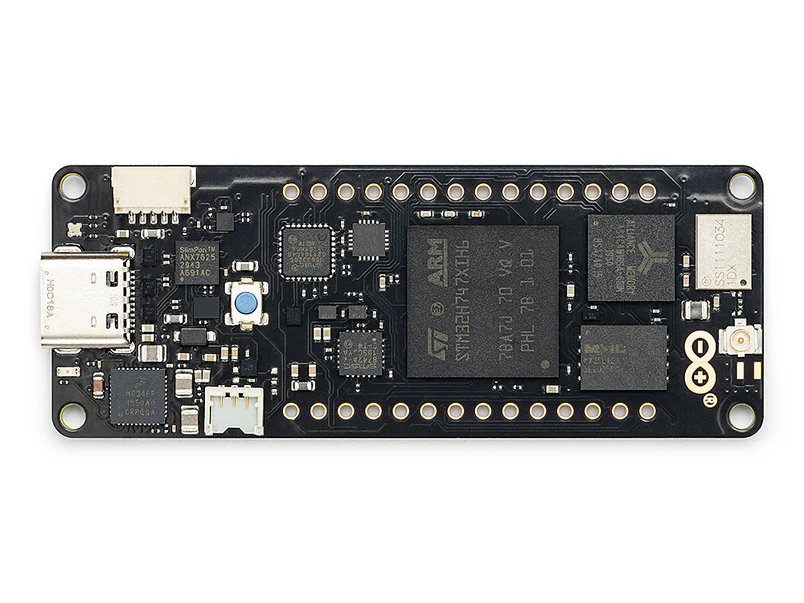
\includegraphics[width=\textwidth]{images/PortentaH7Top.png}
		\vspace{0.2cm}
		\textbf{Figure1: Arduino PortentaH7 Top} \cite{Arduinostore:2024}
		
		\column{0.5\textwidth}
		\centering
		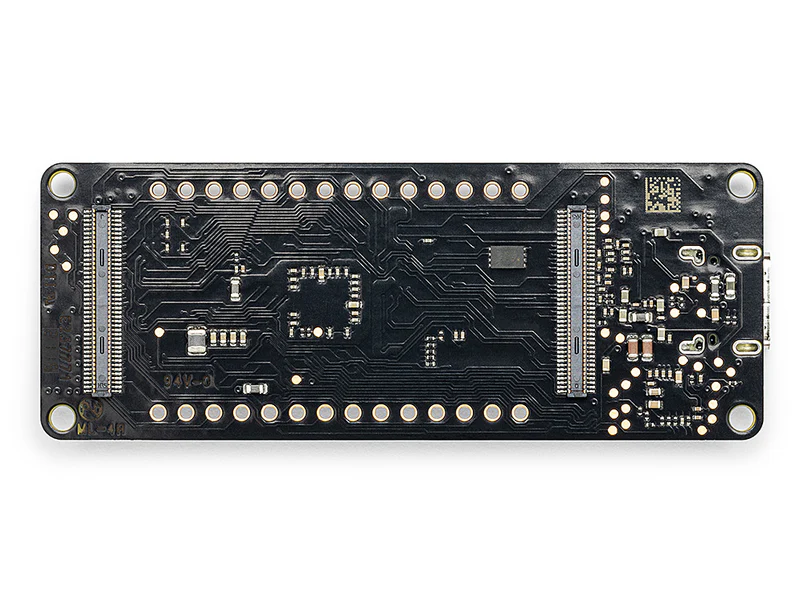
\includegraphics[width=\textwidth]{images/PortentaH7Bottom.png}
		\vspace{0.2cm}
		\textbf{Figure2: PortentaH7 Bottom} \cite{Arduinostore:2024}
	\end{columns}
}


\section{About Cat. M1/NB IoT GNSS Shield}
\STANDARD{About Cat. M1/NB IoT GNSS Shield}
{
	\framesubtitle{Key Features}
\begin{itemize}
	\item \textbf{Connectivity:} LTE Cat M1, NB-IoT for wide area network communication.
	\item \textbf{GNSS:} Supports GPS, GLONASS, Galileo, BeiDou for precise positioning.
	\item \textbf{Low Power:} Optimized for low power consumption, ideal for battery-operated devices.
	\item \textbf{Applications:} Suitable for asset tracking, remote monitoring, and IoT deployments.
\end{itemize}
}

\STANDARD{Portenta H7 Cat. M1/NB IoT GNSS Shield}
{
\begin{columns}
	\column{0.5\textwidth}
	\centering
	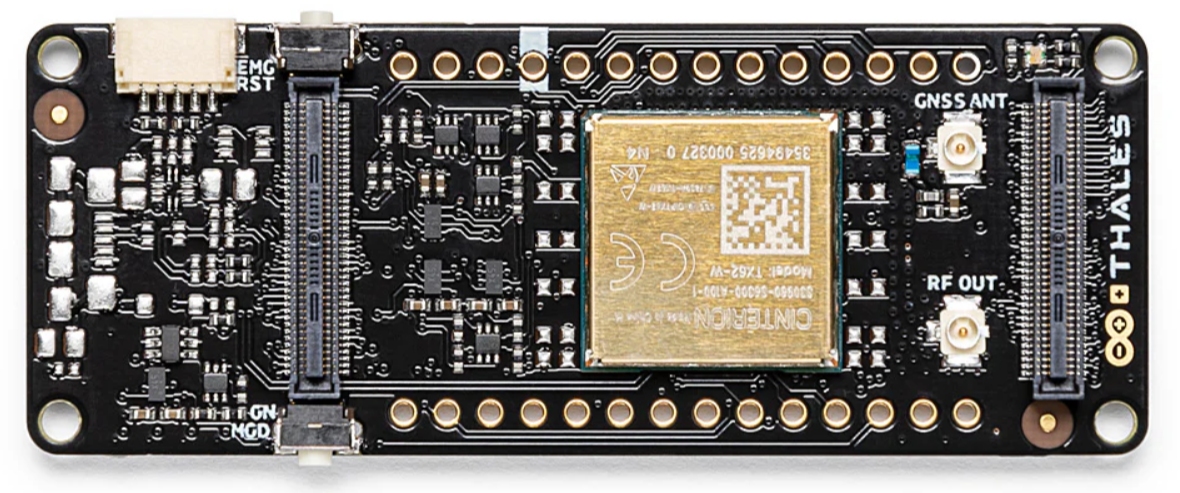
\includegraphics[width=\textwidth]{images/IOTShieldTop.png}
	\vspace{0.2cm}
	\textbf{Figure1: Portenta H7 Cat. M1/NB IoT GNSS Shield TopView} \cite{ArduinoIOTGNSSstore:2024}
	
	\column{0.5\textwidth}
	\centering
	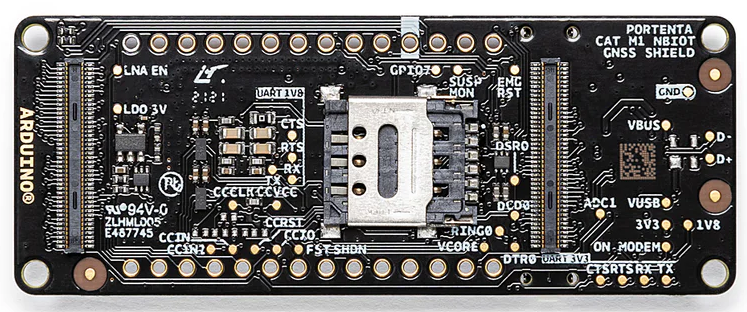
\includegraphics[width=\textwidth]{images/IOTShieldBottom.png}
	\vspace{0.2cm}
	\textbf{Figure2: Portenta H7 Cat. M1/NB IoT GNSS Shield BottomView} \cite{ArduinoIOTGNSSstore:2024}
\end{columns}
}

\section{Benefits of Integration}
\STANDARD{Benefits of Integration}
{ 
	\framesubtitle{Benefits of Integration}
\begin{itemize}
	\item \textbf{Enhanced Connectivity:}
	\begin{itemize}
		\item Multiple network options including cellular and Wi-Fi.
		\item Reliable communication in remote areas.
	\end{itemize}
	\item \textbf{Real-time Geolocation:}
	\begin{itemize}
		\item Accurate tracking of devices in motion.
		\item Useful for logistics and fleet management.
	\end{itemize}
	\item \textbf{Low Power Consumption:}
	\begin{itemize}
		\item Extends battery life for IoT devices.
		\item Suitable for remote and long-term deployments.
	\end{itemize}
	\item \textbf{Industrial and Remote Applications:}
	\begin{itemize}
		\item Monitoring environmental conditions in agriculture.
		\item Tracking assets in supply chain management.
	\end{itemize}
\end{itemize}
}

\section{Technical Specifications}
\STANDARD{Technical Specifications}
{
	\framesubtitle{Technical Specifications}
\begin{itemize}
	\item \textbf{Portenta H7:} \cite{ArduinoPortentaH7:2024}
	\begin{itemize}
		\item Processor: Dual-core ARM Cortex-M7 (480 MHz) and Cortex-M4 (240 MHz).
		\item Memory: 8MB SDRAM, 16MB NOR Flash, 1MB SRAM.
		\item Connectivity: Wi-Fi, Bluetooth, Ethernet, USB, CAN, and more.
		\item Operating Temperature: -40 to +85 degrees Celsius.
	\end{itemize}
	\item \textbf{Cat. M1/NB IoT GNSS Shield:} \cite{ArduinoIOTShield:2024}
	\begin{itemize}
		\item Modem: LTE Cat M1, NB-IoT for IoT applications.
		\item GNSS: Supports GPS, GLONASS, Galileo, BeiDou.
		\item Power Consumption: Ultra-low power, ideal for battery-operated devices.
		\item Antenna: External antenna for improved signal reception.
	\end{itemize}
\end{itemize}	
}

\section{Integration Process}
\STANDARD{Integration Process}
{
	\framesubtitle{Integration Process}
  \textbf{Hardware Connection:}
\begin{itemize}
	\item Stack the Cat. M1/NB IoT GNSS Shield on top of the Portenta H7.
	\item Ensure secure connection of pins and proper alignment.
\end{itemize}
\textbf{Software Setup:}
\begin{itemize}
	\item Install necessary libraries in the Arduino IDE.
	\item Configure settings for cellular and GNSS functionalities.
\end{itemize}
\textbf{Writing and Uploading Code:}
\begin{itemize}
	\item Develop code to handle connectivity and data transmission.
	\item Upload the code to the Portenta H7 and test the integration.
\end{itemize}	
}

\section{Project}
\STANDARD{Project: Real-time GPS Tracker}
{ 
	\framesubtitle{Sample Project: Real-time GPS Tracker}
	The goal of this project is to create a real-time GPS tracker using the Portenta H7 microcontroller board and the Cat. M1/NB IoT GNSS Shield. The tracker will capture GPS coordinates (latitude, longitude, and altitude) and send this data over a cellular network to a remote server.
\textbf{Hardware and Software Requirements:}
\begin{itemize}
	\item Portenta H7
	\item Portenta Cat. M1/NB IoT GNSS Shield
	\item A GPS active antenna (e.g GPS active antenna 28dB) connected to the GNS ANT antenna connector on the top side of the shield.
	\item Connector converter for the active GPS antenna to the board, Coaxial to SMA
	\item SIM card (standard pre-paid or post-paid SIM card that supports
	Cat M1 or NB-IoT connectivity, along with details of APN settings
	and PIN code usually 0000 or 1234. These are usually provided by
	your SIM card provider)
	\item Arduino IDE
\end{itemize} 

\textbf{Procedure}
\begin{itemize}
	\item Stack the Cat. M1/NB IoT GNSS Shield on the Portenta H7.
	\item Attach the GNSS antenna to the shield.
	\item Insert the SIM card with a data plan into the shield.	
\end{itemize} 

	\begin{columns}
		\column{0.5\textwidth}
		\centering
		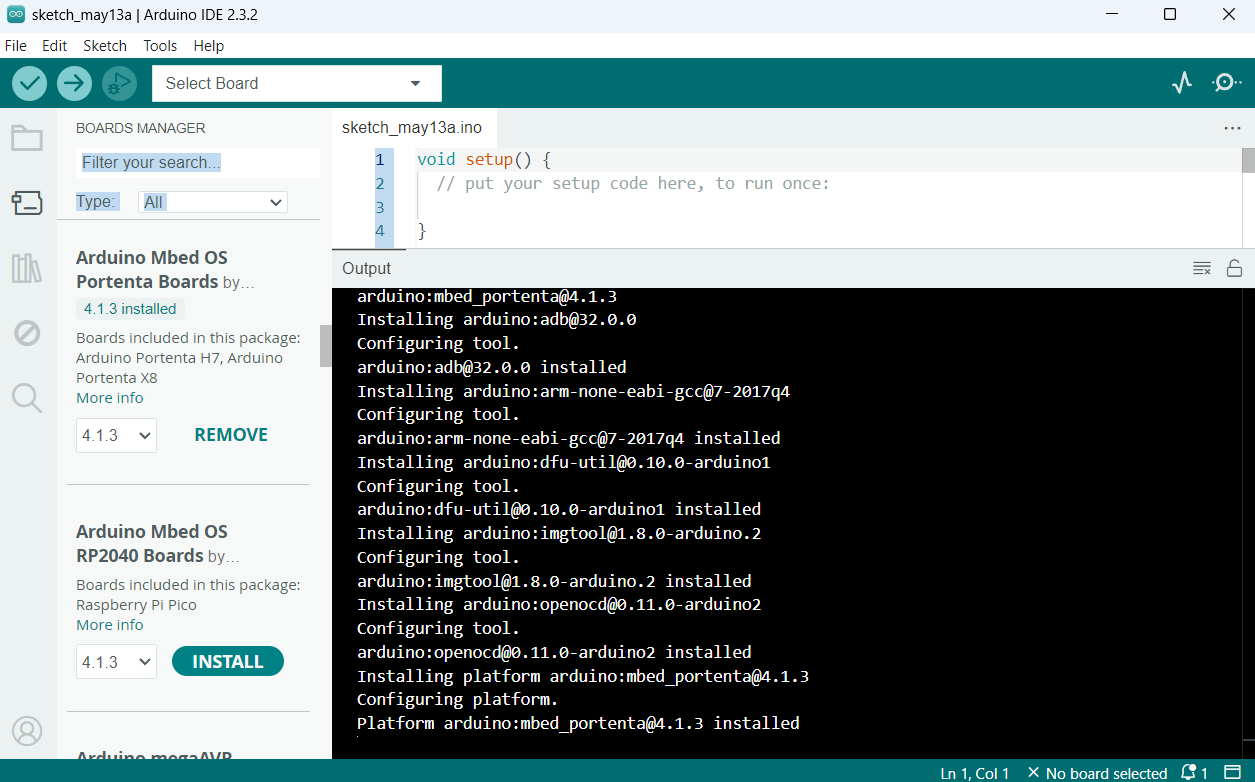
\includegraphics[width=\textwidth]{images/CoreInstallation.png}
		\vspace{0.2cm}
		\textbf{Figure1: Mbed Core Installation} 
		\label{Core}
		
		\column{0.5\textwidth}
		\centering
		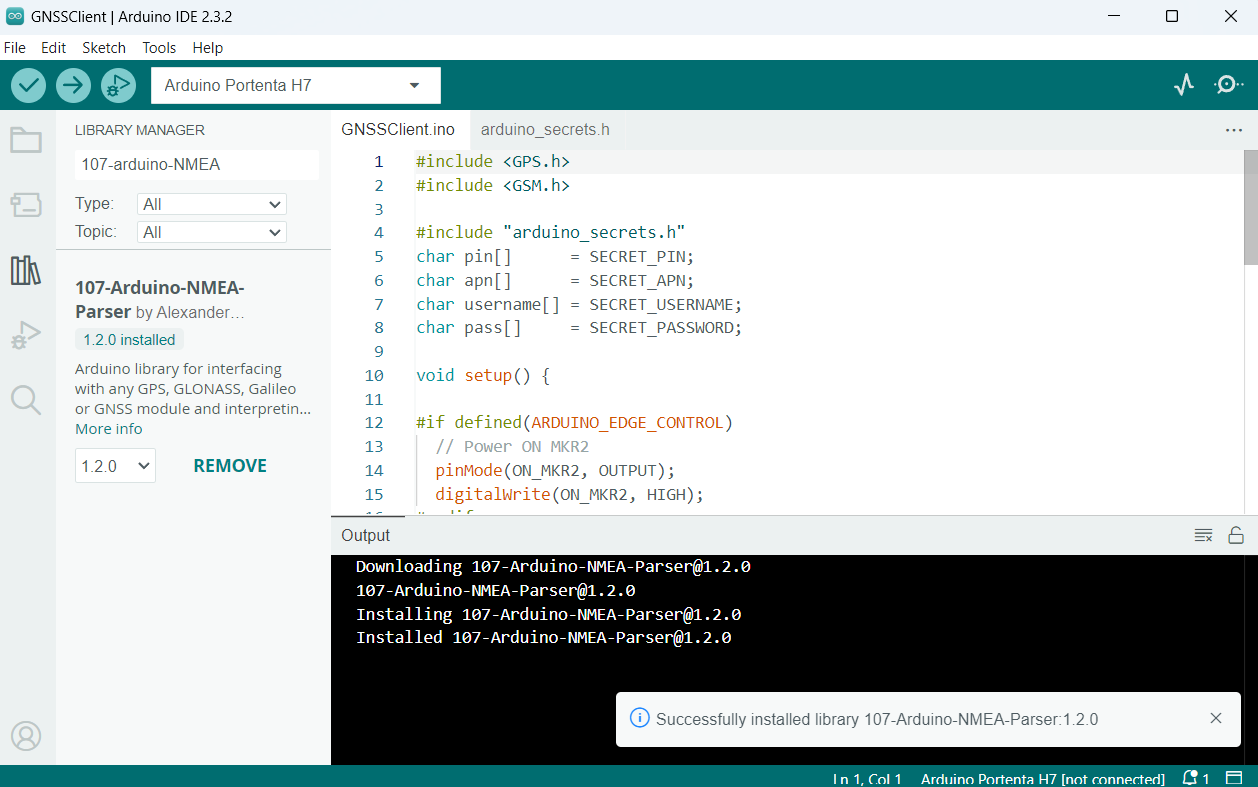
\includegraphics[width=\textwidth]{images/NMEALibraryInstall.png}
		\vspace{0.2cm}
		\textbf{Figure2: NMEA Library Installation} 
		\label{NMEA}
	\end{columns}

\textbf{Arduino IDE}

Make sure that you have the latest Arduino Mbed OS Portenta core installed. You can install it with the board manager under \SHELL{Tools > Board > Board Manager} ~\ref{Core}. With the core installed and the board selected, navigate to \SHELL{File > Examples > GSM > GNSSClient}. You will open an sketch that connects to the SIM card provider and initializes the active GPS antenna. At this point, it will print out GPS readings.

Make sure you go to the arduino\_secrets.h tab and:

\begin{itemize}
	\item Add the PIN of the SIM card you are using and store it in the variable \PYTHON{SECRET\_PIN}.
	\item Browse your IT provider and check the mobile APN link, e.g "online.provider.com" save it inside the \PYTHON{SECRET\_APN}
\end{itemize} 

After finishing this setup, compile and upload the program. We will see the NMEA data in the Serial Monitor.
}

\begin{frame}[fragile]{GNSS Client}
	
	\begin{lstlisting}[language=Python]
	#include <GPS.h>
	#include <GSM.h>
	#include "arduino_secrets.h"
	char pin[]      = SECRET_PIN;
	char apn[]      = SECRET_APN;
	char username[] = SECRET_USERNAME;
	char pass[]     = SECRET_PASSWORD;
		
	void setup() {
		
		#if defined(ARDUINO_EDGE_CONTROL)
		// Power ON MKR2
		pinMode(ON_MKR2, OUTPUT);
		digitalWrite(ON_MKR2, HIGH);
		#endif
		Serial.begin(115200);
		while (!Serial) {}
		// To enable AT Trace debug uncomment the following lines
		\end{lstlisting}
\end{frame}

\begin{frame}[fragile]{GNSS Client}
	
	\begin{lstlisting}[language=Python]
		//GSM.trace(Serial);
		//GSM.setTraceLevel(4);
		Serial.println("Starting Carrier Network registration");
		if(!GSM.begin(pin, apn, username, pass, CATNB)){			Serial.println("The board was not able to register to the network...");
			// do nothing forevermore:
			while(1);
		}
		Serial.println("\nEnable GNSS Engine...");
		// GPS.begin() start and eanble the GNSS engine
		GPS.begin();
		Serial.println("\nGNSS Engine enabled...");	
		}
		\end{lstlisting}
\end{frame}

\begin{frame}[fragile]{GNSS Client}
	
	\begin{lstlisting}[language=Python]
	void loop() {
		// Print out raw NMEA strings.
		// For parsed output look at the MicroNMEA_integration example.
		if(GPS.available()){
			Serial.print((char) GPS.read());
			delay(1);
		}
		// After geting valid packet GPS.end() can be used to stop and
		// disable the GNSS engine
		// GPS.end();
	}
		
	\end{lstlisting}
\end{frame}

\STANDARD{Parse NMEA GPS Sentences}
{
	\begin{itemize}
	\item It was not possible to evaluate those messages (NMEA sentences) of GPS data in Serial Monitor. So we need a NMEA Parser to convert messages received from the GPS modem, parsing and saving them into variables.
	\item In this way, it is possible to interact with the data that you need for your application, for instance getting only latitude and longitude. You will be able to save those values into variables, instead of having the whole NMEA messages.
	\item Go to \SHELL{Sketch > Include Library > 107-Arduino-NMEA-Parser library} ~\ref{NMEA} and Install.
	\item Open the example from the library at \SHELL{Examples > 107-Arduino-NMEA-Parser > NMEA-Basic} and modify accordingly
	\end{itemize}
}


\begin{frame}[fragile]{Include the libraries}
	
	\begin{lstlisting}[language=Python]
		#include "GPS.h"
		#include "GSM.h"
		#include "ArduinoNmeaParser.h"
		#include "Arduino_secrets.h"
		
		char pin[]      = SECRET_PIN;
		char apn[]      = SECRET_APN;
		char username[] = SECRET_LOGIN;
		char pass[]     = SECRET_PASS;
	\end{lstlisting}
\end{frame}

\begin{frame}[fragile]{Inside the setup() initialize the GSM and GPS modules}
	
	\begin{lstlisting}[language=Python]
void setup(){
	Serial.begin(115200);
	while (!Serial) {}
	Serial.println("GSM...");
	GSM.begin(pin, apn, username, pass, CATNB);
	Serial.println("GPS...");
	GPS.begin();
	Serial.println("Success");
}
	\end{lstlisting}
\end{frame}

\begin{frame}[fragile]{Edit the loop to parse the GPS readings instead of the Serial1}
	
	\begin{lstlisting}[language=Python]
void loop(){
	while(GPS.available()){
		parser.encode((char)GPS.read());
	}
}
	\end{lstlisting}
\end{frame}


\section{Use Cases and Applications}
\STANDARD{Use Cases and Applications}
{
	\framesubtitle{Use Cases and Applications}
	\begin{itemize}
		\item \textbf{Asset Tracking:}
		\begin{itemize}
			\item Real-time location monitoring.
			\item Reduces loss and improves asset management.
		\end{itemize}
		\item \textbf{Remote Monitoring and Control:}
		\begin{itemize}
			\item Monitor environmental conditions remotely.
			\item Control devices and machinery from a distance.
		\end{itemize}
		\item \textbf{Environmental Monitoring:}
		\begin{itemize}
			\item Track weather conditions, air quality, and other environmental factors.
			\item Useful for smart agriculture and urban planning.
		\end{itemize}
		\item \textbf{Smart Agriculture:}
		\begin{itemize}
			\item Monitor soil moisture, crop health, and livestock tracking.
			\item Optimize resource usage and improve yield.
		\end{itemize}
		\item \textbf{Industrial IoT:}
		\begin{itemize}
			\item Monitor and control industrial processes.
			\item Enhance efficiency and reduce downtime.
		\end{itemize}
	\end{itemize}
}